\documentclass[12pt]{beamer}
\usepackage{cmap}
\usepackage[T2A]{fontenc}
\usepackage[utf8]{inputenc}
\usepackage{ifluatex}
\usefonttheme[onlymath]{serif}
\usepackage{svg}
\usepackage{enumerate}
\usepackage{hyperref}
\usepackage{mathtools}
\setbeamertemplate{footline}[frame number]
\definecolor{beamer@darkgreen}{rgb}{0,0.6,0}
\setbeamercolor{normal text}{fg=black,bg=white}
\setbeamercolor{title}{fg=black,bg=beamer@darkgreen}
\setbeamercolor{frametitle}{fg=black,bg=beamer@darkgreen}
\setbeamercolor{background canvas}{parent=normal text}

\usepackage[english,russian]{babel}
\usepackage{graphicx}
\usepackage{listings}
\DeclareMathOperator{\sign}{sign}

\usepackage{enumerate}

\author{Катя Тузова}
\title{Машинное обучение}
\date{}

\usepackage{gensymb}

\subtitle{Лекция 8. Логические алгоритмы классификации.}

\begin{document}	
\frame{\titlepage}

\begin{frame}\frametitle{Разбор летучки}
Какие условия должны выполняться для того, чтобы объект считался опорным?
\end{frame}

\begin{frame}\frametitle{Обзор уже известных подходов}
\begin{enumerate} 
	\item Метрический
		\begin{enumerate} [--]
			\item K ближайших соседей
			\item Кластеризация 
		\end{enumerate}
	\item Линейный
		\begin{enumerate} [--]
			\item Градиентный спуск
			\item Метод опорных векторов
		\end{enumerate}
\end{enumerate}
\end{frame}

\begin{frame}\frametitle{Логические закономерности}
${X^l = \left( x_i, y_i \right)_{i=1}^l}$ - обучающая выборка.\\
\vspace{5mm}
Логическая закономерность (правило) -- предикат ${\beta: X \rightarrow \left\{ 0, 1 \right\} }$, который удовлетворяет двум требованиям:\\
\begin{enumerate} [-]
	\item Интерпретируемость
	\item Информативность относительно одного из классов ${c \in Y}$
\end{enumerate}
\vspace{5mm}
Алгоритм: $a(X, \beta) \rightarrow y$
\end{frame}


\begin{frame}\frametitle{Интерпретируемость}
	\begin{enumerate} [-]
		\item Записывается на естественном языке
		\item Зависит от небольшого числа признаков
	\end{enumerate}
\end{frame}

\begin{frame}\frametitle{Интерпретируемость}
Медицинская диагностика:	
	\begin{enumerate} [-]
		\item Температура выше n\degree
		\item Есть кашель
	\end{enumerate}
\vspace{5mm}
Кредитный скоринг:	
	\begin{enumerate} [-]
		\item Заработная плата выше, чем $n$ руб.
		\item Кредит не больше, чем $m$ руб.
	\end{enumerate}
\end{frame}

\begin{frame}\frametitle{Интерпретируемость}
\begin{figure}[htbp]
  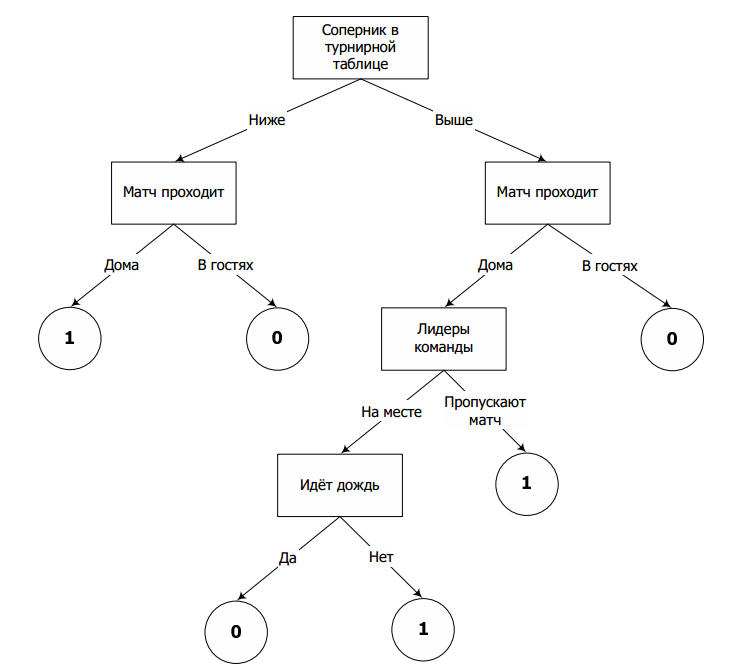
\includegraphics[height=190pt, keepaspectratio = true]{images/dtree}   
\end{figure}
\end{frame}

\begin{frame}\frametitle{Информативность}
	\begin{itemize}
		\item[--] Максимизировать количество правильно распознанных объектов класса $c$\\
		${ tp(\beta) = \# \left\{ x_i: \beta(x_i) = 1 , y_i = c \right\} \rightarrow \max }$\\

		\item[--] Минимизировать количество объектов, ошибочно классифицированных как класс $c$\\
		${ fp(\beta) = \# \left\{ x_i: \beta(x_i) = 1 , y_i \neq c \right\} \rightarrow \min }$\\
		
	\end{itemize}
\end{frame}

\begin{frame}\frametitle{Информативность}
\begin{figure}[htbp]
  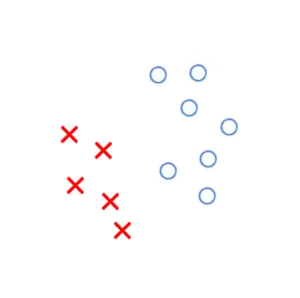
\includegraphics[height=190pt, keepaspectratio = true]{images/dtree_1}   
\end{figure}
\end{frame}

\begin{frame}\frametitle{Информативность}
\begin{figure}[htbp]
  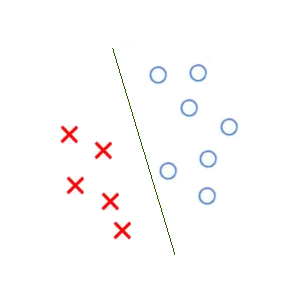
\includegraphics[height=190pt, keepaspectratio = true]{images/dtree_2}   
\end{figure}
\end{frame}

\begin{frame}\frametitle{Информативность}
\begin{figure}[htbp]
  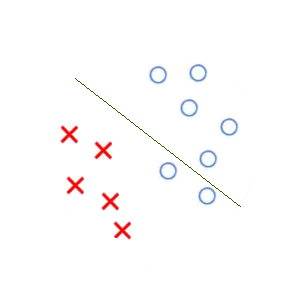
\includegraphics[height=190pt, keepaspectratio = true]{images/dtree_3}   
\end{figure}
\end{frame}

\begin{frame}\frametitle{Информативность}
\begin{figure}[htbp]
  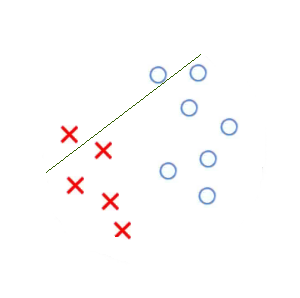
\includegraphics[height=190pt, keepaspectratio = true]{images/dtree_4}   
\end{figure}
\end{frame}

\begin{frame}\frametitle{Поиск закономерности}
\begin{figure}[htbp]
  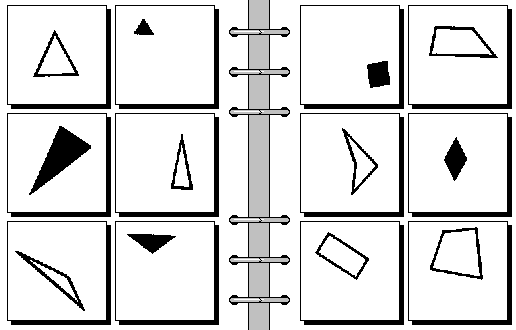
\includegraphics[height=150pt, keepaspectratio = true]{images/bongard6}   
\end{figure}
\end{frame}

\begin{frame}\frametitle{Поиск закономерности}
\begin{figure}[htbp]
  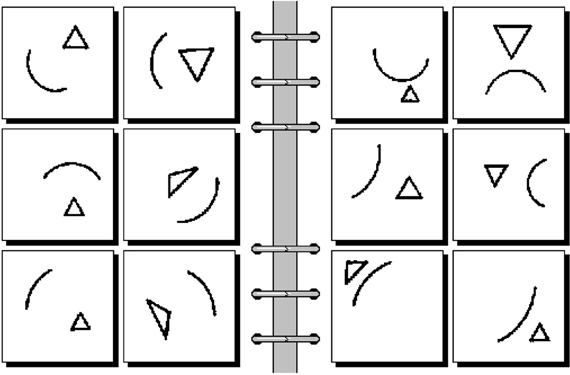
\includegraphics[height=150pt, keepaspectratio = true]{images/bongard40}   
\end{figure}
\end{frame}

\begin{frame}\frametitle{Поиск закономерности}
\begin{figure}[htbp]
  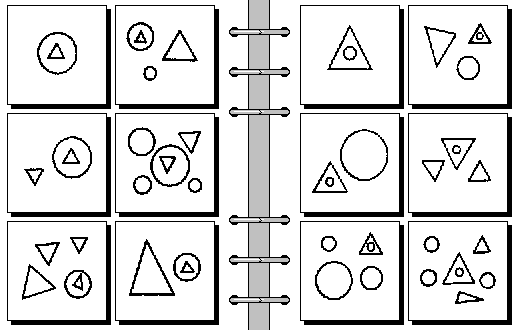
\includegraphics[height=150pt, keepaspectratio = true]{images/bongard47}   
\end{figure}
\end{frame}

\begin{frame}\frametitle{Поиск закономерности}
\begin{figure}[htbp]
  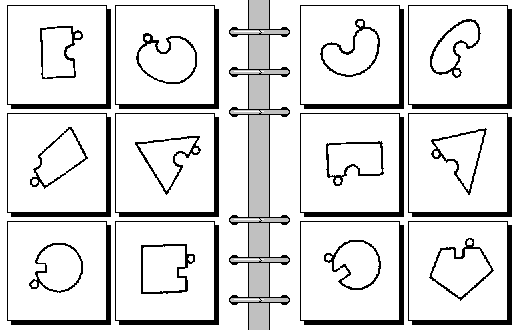
\includegraphics[height=150pt, keepaspectratio = true]{images/bongard55}   
\end{figure}
\end{frame}

\begin{frame}\frametitle{Основные вопросы}
	\begin{itemize}
		\item[--] Как изобретать признаки? 
		\item[--] Какого вида закономерности $\beta(x)$ нужны?
		\item[--] Как определять информативность? 
		\item[--] Как выбирать закономерности?
		\item[--] Как объединять закономерности в алгоритм?
	\end{itemize}
\end{frame}

\begin{frame}\frametitle{Как изобретать признаки}
Какие признаки выбрать для задачи кредитного скоринга?
\end{frame}

\begin{frame}\frametitle{Виды правил}
\end{frame}

\begin{frame}\frametitle{Виды правил}
\begin{itemize}
\item[--] Пороговое условие (decision stump)\\
$\beta(x) = \left[f_j(x) \leq a_j \right]$ или  $\left[a_j \leq f_j(x) \leq b_j \right]$
\item[--] Конъюнкция $J$ пороговых условий
$\beta(x) = \bigwedge\limits_{j \in J} \left[a_j \leq f_j(x) \leq b_j \right]$
\item[--] Синдром -- выполнение не менее $d$ условий из $J$
$\beta(x) = \left[\sum\limits_{j \in J} \left[a_j \leq f_j(x) \leq b_j \right] \geq d \right]$
\end{itemize}
\end{frame}

\begin{frame}\frametitle{Оценивание информативности}
Идея: Хотим получить один критерий из двух:\\
\vspace{5mm}
${ tp(\beta) = \# \left\{ x_i: \beta(x_i) = 1 , y_i = c \right\} \rightarrow \max  }$ 
${ fp(\beta) = \# \left\{ x_i: \beta(x_i) = 1 , y_i \neq c \right\} \rightarrow \min}$ \\
\vspace{5mm}
	Очевидные свертки:\\
	\begin{itemize}
		\item[--] $I(tp, fp) = \frac{tp}{tp+fp} \rightarrow \max$
		\item[--] $I(tp, fp) = tp-fp \rightarrow \max$
		\item[--] $I(tp, fp) = tp-Cfp \rightarrow \max$			
	\end{itemize}
\end{frame}

\begin{frame}\frametitle{Пример свертки двух критериев}
Пусть число примеров искомого класса 200 и число остальных объектов 100\\
\vspace{5mm}
\begin{tabular}{|r l|l|l|l|}
  \hline 
  $tp$ & $fp$ & $tp-fp$ & $tp-5fp$ & $\frac{tp}{tp+fp}$\\ 
  \hline \hline
  50 & 0 & \textcolor{red}{50} & 50 & 1\\
  \hline
  100 & 50 & \textcolor{red}{50} & -150 & 0.6\\
  \hline \hline
  50 & 9 & 41 & \textcolor{red}{5} & \textcolor{red}{0.84}\\
  \hline  
  5 & 0 & 5 & \textcolor{red}{5} & \textcolor{red}{1}\\  
  \hline 
\end{tabular}
\end{frame}

\begin{frame}\frametitle{Используемые критерии информативности}
\begin{enumerate}[--]
\item Энтропийный информационный критерий\\
$IGain(tp,fp) = h(\frac{P}{l}) - \frac{tp+tp}{l}h(\frac{tp}{tp+fp}) - \frac{l-tp-fp}{l}h(\frac{P-tp}{l-tp-fp}) \rightarrow \max$\\
где $h(q) = -q\log_2q - (1-q)\log_2(1-q)$
\item Критерий Джини\\
$IGini(tp,fp)=IGain(tp,fp)$, где $h(q)=4q(1-q)$
\item Fisher’s Exact Test\\
$IStat(tp,fp) = -\frac{1}{l}\log_2\frac{C_P^{tp}C_N^{fp}}{C_{P+N}^{tp+fp}} \rightarrow \max$
%\item Критерий Донского\\
%$I(\beta,X^l)= \# \left\{ (x_i, x_j): \beta(x_i) \neq \beta(x_j), y_i \neq y_j \right\}$

%\item Gini impurity\\
%$IGini(p,n)=IGain(p,n)$, где $h(q)=4q(1-q)$
%\item Boosting\\
%$\sqrt{p} - \sqrt{n} \rightarrow \max$
\end{enumerate}
\vspace{5mm}
$P$ - общее количество объектов искомого класса\\
 $N$ -- количество остальных объектов
\end{frame}

%\begin{frame}\frametitle{Закономерности в pn области}
%\textcolor{red}{TODO: картинка}
%\end{frame}



\begin{frame}\frametitle{Поиск информативных закономерностей}
Input: Обучающая выборка $X^l$\\
Output: Множество закономерностей $\mathcal{B}$\\
\vspace{5mm}
Выбрать начальное множество $\mathcal{B}$\\
Повторять пока правила улучшаются:\\
\hspace{10mm} $\mathcal{B}'=$ множество модификаций правил $\beta \in \mathcal{B}$\\
\hspace{10mm} Удалить слишком похожие правила из $\mathcal{B} \cup \mathcal{B}'$\\
\hspace{10mm} Оценить инфомативность правил $\beta \in \mathcal{B}'$\\
\hspace{10mm} $\mathcal{B}=$ наиболее информативные правила из $\mathcal{B} \cup \mathcal{B}'$\\
\vspace{5mm}
Примеры:\\
\begin{enumerate}[--]
	\item Генетические алгоритмы
	\item Метод ветвей и границ	
	\item Стохастический локальный поиск	
\end{enumerate}

\end{frame}

\begin{frame}\frametitle{Критерий Парето}
Парето-фронт -- множество недоминируемых закономерностей (правее и ниже точек нет)
\begin{figure}[htbp]
  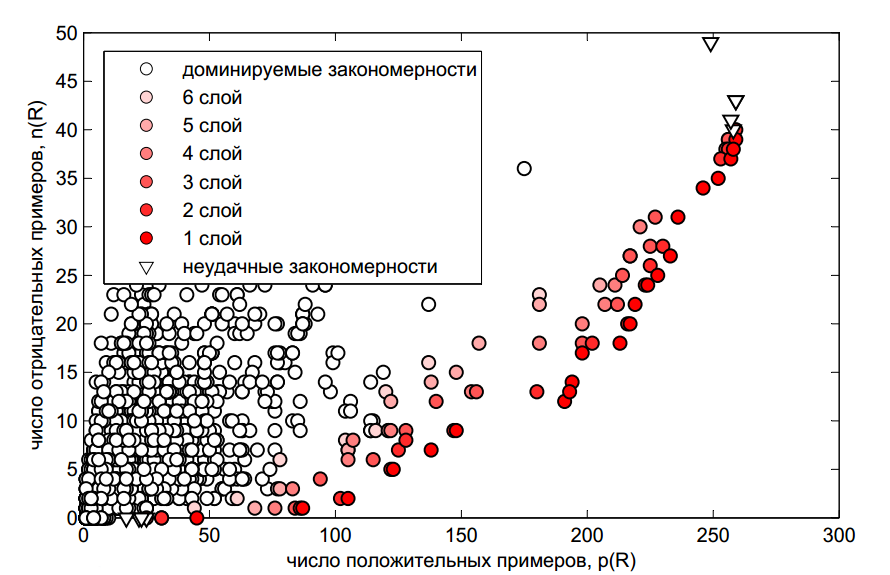
\includegraphics[height=150pt, keepaspectratio = true]{images/pareto}   
\end{figure}
\footnotesize\textcolor{gray} {Картинка с machinelearning.ru}
\end{frame}

\begin{frame}\frametitle{Вопрос}
Как собрать классификатор из закономерностей?
\end{frame}

\begin{frame}\frametitle{Решающий список}
Множество классов $c_1,c_2,\dots, c_T \in Y$\\
\vspace{5mm}
Идея:\\
Возьмем $\beta_1(x), \beta_2(x), \dots, \beta_T(x)$ закономерностей и будем по порядку применять на объекте. 
Как только предикат $\beta_i$ сработал -- вернем соответствующий класс $c_i$.
\end{frame}

\begin{frame}\frametitle{Решающий список}
Множество классов $c_1,c_2,\dots, c_T \in Y$\\
\vspace{5mm}
Идея:\\
Возьмем $\beta_1(x), \beta_2(x), \dots, \beta_T(x)$ закономерностей и будем по порядку применять на объекте. 
Как только предикат $\beta_i$ сработал -- вернем соответствующий класс $c_i$.\\
\vspace{5mm}
$E(\beta_i, X^l) = \frac{fp(\beta_i)}{fp(\beta_i)+tp(\beta_i)} \rightarrow \min$ -- доля ошибок $\beta_i$ на $X^l$\\
\vspace{5mm}
Т.к. каждое правило принимает окончательное решение $\Rightarrow$ ошибка правила равна ошибке всего алгоритма
\end{frame}

%\begin{frame}\frametitle{Жадный алгоритм для решающего списка}
%Input: $X^l$, семейство предикатов $\mathcal{B}$, $T_{max}$, $I_{min}$, $E_{max}$, $l_0$\\
%Output: Решающий список $\left\{ \beta_i, c_i \right\}_{i=1}^T$\\
%\vspace{5mm}
%$U = X^l$\\
%Для всех $i = 1,2,\dots,T_{max}$\\
%\hspace{10mm} Выбрать класс $c_i$\\
%\hspace{10mm} Максимизировать информативность при \\
%\hspace{40mm} ограничении на число ошибок\\
%\hspace{10mm} Если $I(\beta_i, U) < I_{min}$ продолжить\\
%\hspace{10mm} Убрать объекты, покрытые правилом $\beta_i$\\
%\hspace{10mm} Если $\vert U \vert \leq l_0$ выйти
%\end{frame}

\begin{frame}\frametitle{Жадный алгоритм для решающего списка}
Input: $X^l$, семейство предикатов $\mathcal{B}$, $T_{max}$, $I_{min}$, $E_{max}$, $l_0$\\
Output: Решающий список $\left\{ \beta_i, c_i \right\}_{i=1}^T$\\
\vspace{5mm}
$U = X^l$\\
Для всех $i = 1,2,\dots,T_{max}$\\
\hspace{10mm} Выбрать класс $c_i$\\
\hspace{10mm} $\beta_i = \max\limits_{E(\beta, U) \leq E_{max}} I(\beta, U)$\\
\hspace{10mm} Если $I(\beta_i, U) < I_{min}$ продолжить\\
\hspace{10mm} $U = \left\{ x \in U: \beta_i(x) = 0 \right\}$\\
\hspace{10mm} Если $\vert U \vert \leq l_0$ выйти
\end{frame}

\begin{frame}\frametitle{Наблюдения}
\begin{enumerate}[--]
\item Низкое качество классификации
\item Разные стратегии выбора класса $c_i$
\item Подбор параметров
\end{enumerate}
\end{frame}

\begin{frame}\frametitle{Наблюдения}
\begin{enumerate}[--]
\item Низкое качество классификации
\item Разные стратегии выбора класса $c_i$
\item Подбор параметров
\end{enumerate}
\vspace{5mm}
Параметр $E_{max}$ влияет на сложность списка:\\
$E_{max} \downarrow$ $\Rightarrow$ $tp(\beta_i) \downarrow$, $T \uparrow$\\
$E_{max} \uparrow$, $T_{max} \uparrow$ $\Rightarrow$ underfitting
\end{frame}

\begin{frame}\frametitle{Бинарное решающее дерево}
Бинарное решающее дерево -- алгоритм классификации $a(x, \beta)$, задающийся бинарным деревом:\\
\begin{enumerate}[--]
\item $\forall v \in V_{inner} \rightarrow \beta_v: X \rightarrow \left\{ 0,1\right\}$, $\beta \in \mathcal{B}$
\item $\forall v \in V_{leaf} \rightarrow $ имя класса $c_v \in Y$\\

\begin{figure}[htbp]
  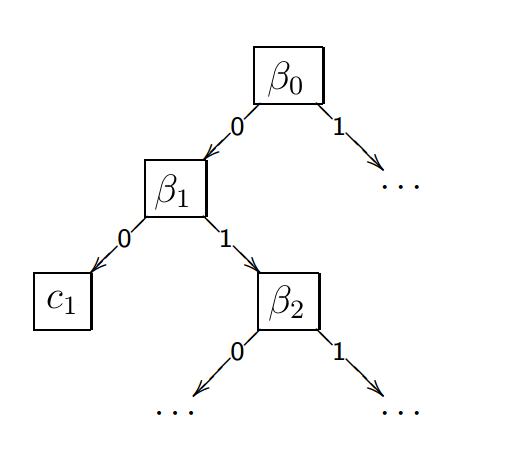
\includegraphics[height=150pt, keepaspectratio = true]{images/binary_tree}   
\end{figure}
\end{enumerate}
\end{frame}

\begin{frame}\frametitle{Пример решающего дерева}
\begin{figure}[htbp]
  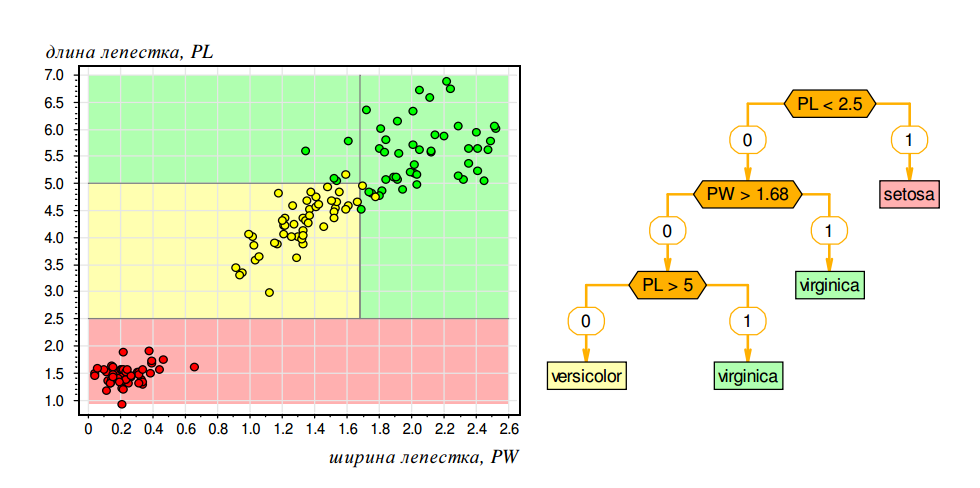
\includegraphics[height=150pt, keepaspectratio = true]{images/fisher}   
\end{figure}
В осях двух самых информативных признаков (из 4)
два класса разделились без ошибок, на третьем 3 ошибки.
\footnotesize\textcolor{gray} {Картинка с machinelearning.ru}

\end{frame}

\begin{frame}\frametitle{Набор конъюнкций}
\begin{figure}[htbp]
  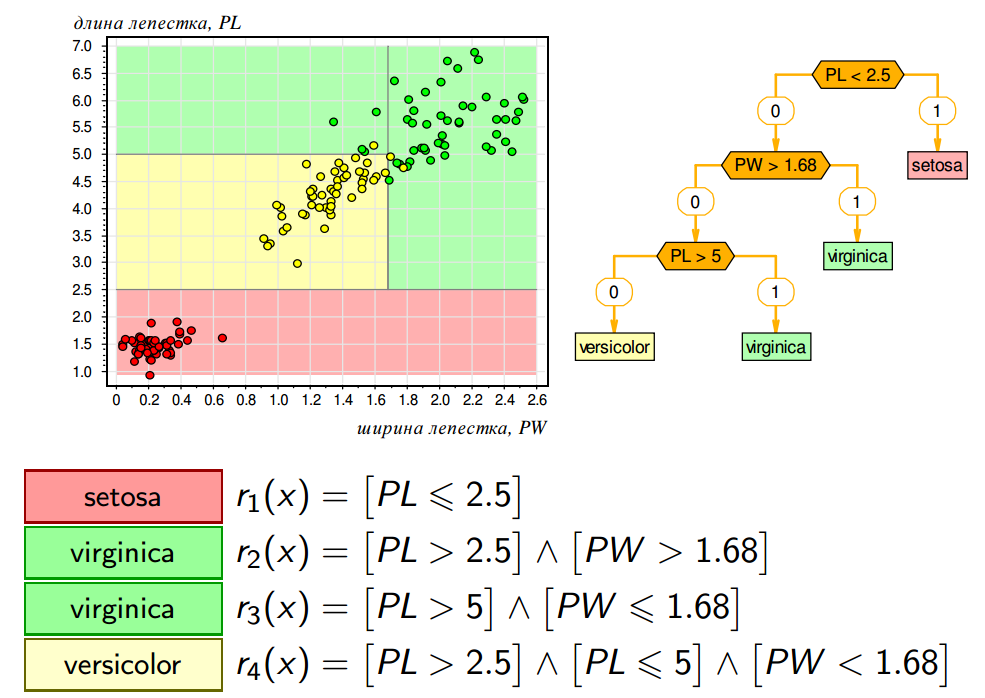
\includegraphics[height=190pt, keepaspectratio = true]{images/fisher1}   
\end{figure}
\footnotesize\textcolor{gray} {Картинка с machinelearning.ru}

\end{frame}

%\begin{frame}\frametitle{Алгоритм построения ID3}
%Input: $X^l$, $\mathcal{B}$\\
%Output: Решающее дерево \\
%\vspace{3mm}
%Если все объекты из $U$ лежат в одном классе $c \in Y$,\\ 
%\hspace{10mm} вернуть новый лист $v$, $c_v = c$\\
%Найти предикат с максимальной информативностью\\
%Разбить выборку на две части $U = U_0 \cup U_1$ по предикату $\beta$\\
%Если $U_0$ или $U_1$ пуст, то вернуть новый лист $v$,\\ $c_v$ = Мажоритарный класс(U)\\
%Создать новую внутреннюю вершину $v$: $\beta_v = \beta$\\
%Рекурсивно построить левое и правое поддеревья
%\end{frame}

\begin{frame}\frametitle{Алгоритм построения ID3}
LearnID3 (U, $\mathcal{B}$):\\
\hspace{10mm} Если все объекты из $U$ лежат в одном классе $c \in Y$: \\
\hspace{20mm} Вернуть новый лист $v$, $c_v = c$\\
\vspace{3mm}
\hspace{10mm} $\beta^* = \max\limits_{\beta \in \mathcal{B}} I(\beta, U)$\\
\vspace{3mm}
\hspace{10mm} $U_0 = \left\{ x \in U : \beta^*(x) = 0\right\}$	\\
\hspace{10mm} $U_1 = \left\{ x \in U : \beta^*(x) = 1\right\}$	\\
\vspace{3mm}
\hspace{10mm} Если $U_0 = \oslash$ или $U_1 = \oslash$:\\ 
\hspace{20mm} Вернуть $v$, $c_v$ = Majority(U)\\
\vspace{3mm}
\hspace{10mm} Создать новую внутреннюю вершину $v$: $\beta_v = \beta^*$\\
\vspace{3mm}
\hspace{10mm} $L_v =$ LearnID3 ($U_0$, $\mathcal{B}$)\\
\hspace{10mm} $R_v =$ LearnID3 ($U_1$, $\mathcal{B}$)\\
\hspace{10mm} Вернуть $v$
\end{frame}

\begin{frame}\frametitle{Критерий информативности}
\begin{enumerate}[--]
%\item Отделение одного класса\\
%$I(\beta,X^l) = \max\limits_{c \in Y} I_c (\beta,X^l)$
%\item Многоклассовый энтропийный критерий
%$I(\beta,X^l) = \sum\limits_{c \in Y} h(\frac{P_c}{l}) - \frac{p}{l}h(\frac{p_c}{p}) - \frac{l-p}{l}h(\frac{P_c-p_c}{l-p})$\\
%где $P_c = \# \left\{ x_i: y_i =c \right\} $, $p = \# \left\{ x_i: \beta(x_i)= 1 \right\} $, $h(z) = -z log_2 z$
\item Критерий Джини\\
$I(\beta,X^l)= \# \left\{ (x_i, x_j): \beta(x_i) = \beta(x_j), y_i = y_j \right\}$
\item Критерий Донского\\
$I(\beta,X^l)= \# \left\{ (x_i, x_j): \beta(x_i) \neq \beta(x_j), y_i \neq y_j \right\}$
\end{enumerate}
\end{frame}

\begin{frame}\frametitle{Плюсы и минусы}
\begin{enumerate}[+]
\item Интерпретируемость и простота классификации
\item Допустимы разнотипные данные и данные с пропусками
\item Не бывает отказов от классификации
\item Трудоёмкость линейна по длине выборки
\item Можно варьировать множество $\mathcal{B}$
\end{enumerate}
\begin{enumerate}[-]
\item Жадный ID3 сильно переобучается
\item Высокая чувствительность к шуму, к составу выборки, к критерию информативности
\item Чем дальше $v$ от корня, тем меньше надёжность выбора $\beta_v$ , $c_v$
\end{enumerate}
\end{frame}

\begin{frame}\frametitle{Переобучение}
\begin{figure}[htbp]
  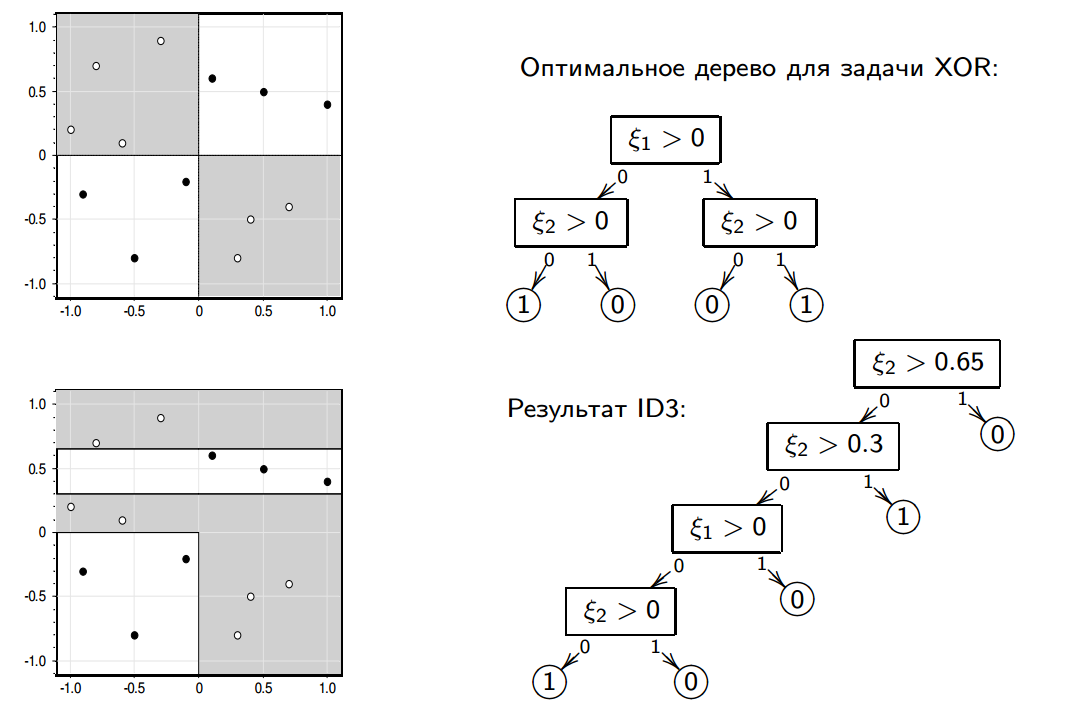
\includegraphics[height=190pt, keepaspectratio = true]{images/overfitting}   
\end{figure}
\vspace{5mm}
\footnotesize\textcolor{gray} {Картинка с machinelearning.ru}
\end{frame}

\begin{frame}\frametitle{Подрезание дерева C4.5}
$X^k$ -- независимая контрольная выборка, $k \approx 0.5l$\\
Для всех $v \in V_{inner}$:\\
\hspace{10mm} $S_v$ = подмножество объектов $X^k$, дошедших до $v$\\
\hspace{10mm} Если $S_v = \oslash$:\\
\hspace{20mm} Вернуть новый лист $v$, $c_v$ = Majority(U)\\
\hspace{10mm} Вычислить число ошибок четырьмя способами:\\
\hspace{20mm} $r(v)$ -- поддеревом, растущим из вершины $v$\\
\hspace{20mm} $r_L(v)$ -- левой дочерней вершины $L_v$\\
\hspace{20mm} $r_R(v)$ -- правой дочерней вершины $R_v$\\
\hspace{20mm} $r_c(v)$ -- к классу $c \in Y$\\
\hspace{10mm} В зависимости от того, какое из них минимально:\\
\hspace{20mm} Сохранить поддерево $v$\\
\hspace{20mm} Заменить поддерево $v$ поддеревом $L_v$\\
\hspace{20mm} Заменить поддерево $v$ поддеревом $R_v$\\
\hspace{20mm} Заменить $v$ листом $c_v = \min\limits_{c \in Y} r_c(v)$\\
\end{frame}

%\begin{frame}\frametitle{Небрежные деревья}
%\textcolor{red}{TODO?}
%Input: Выборка $X^l$, семейство правил $\mathcal{B}$, глубина дерева $H$\\
%Output: условия $\beta_h$, $h = 1, \dots, H$, таблица $T$ : $\left\{0, 1\right\}^H \rightarrow Y$\\
%Для всех $h = 1, \dots, H$:\\
%\hspace{10mm} $\beta_h = \max\limits_{\beta \in \mathcal{B}} I(\beta_1, \dots, \beta_{h-1}, X^l)$\\
%Для всех $b = (b_1, \dots, b_H ) \in {0, 1}$\\
%\hspace{10mm} $T(b_1,\dots, b_H ) = \max\limits_{c \in Y} \sum\limits_{i=1}^l \left[y_i = c\right] \prod\limits_{h=1}^H \left[ %\beta_h(x_i) = b_h \right]$
%\end{frame}

\begin{frame}\frametitle{Композиции алгоритмов}
\begin{enumerate} [--]
\item Можно использовать результаты нескольких	алгоритмов, а не одного.
\item Часто композиция алгоритмов может давать не худший или даже лучший результат
\end{enumerate}
\end{frame}


\begin{frame}\frametitle{Вопрос}
Почему это работает?
\end{frame}

\begin{frame}\frametitle{Почему это работает}
\begin{enumerate} [--]
\item Ошибки	 алгоритмов взаимно компенсируются	
\item На одних объектах хорошо работают одни алгоритмы, на других -- другие	
\end{enumerate}
\end{frame}

\begin{frame}\frametitle{Композиции алгоритмов}
\begin{enumerate} [--]
\item Желательно	 использовать принципиально разные алгоритмы, наборы признаков	
\item Не	 всегда два оптимальных алгоритма в смеси дадут оптимальный результат
\item Чем больше параметров -- тем больше шанс	 переобучиться	
\end{enumerate}
\end{frame}


\begin{frame}\frametitle{Bootstrapping}
Выборка $X^l$\\
\vspace{5mm}
Сгенерируем много датасетов так: будем из $X$ выбирать $l$ объектов с повторениями
\end{frame}

\begin{frame}\frametitle{Баггинг}
Выборка $X^l$\\
\vspace{5mm}
Сделаем путем bootstrapping $M$ датасетов размера $l$, потом обучим $M$ моделей, а потом усредним\\
$y(x) = \frac{1}{M} \sum\limits_{i=1}^l y_i(x)$

\end{frame}

\begin{frame}\frametitle{Бустинг}
\begin{enumerate} [--]
\item Предположим, что у нас есть возможность обучать какую-нибудь простую модель на подмножестве данных.
\item Обучили модель, посмотрели, где она хорошо работает, обучили следующую модель на том подмножестве, где она работает плохо, повторили.
\end{enumerate}
\end{frame}

\begin{frame}\frametitle{Random forest}
Голосование деревьев классификации, $Y = \left\{ -1, +1 \right\}$\\
$a(t) = \sign \frac{1}{T} \sum\limits_{t=1}^T b_t(x)$\\
\begin{enumerate}[--]
\item Каждое дерево $b_t(x)$ обучается по случайной выборке с повторениями
\item В каждой вершине признак выбирается из случайного подмножества $\sqrt{n}$ признаков
\item Признаки и пороги выбираются по критерию Джини
\end{enumerate}
\end{frame}

\begin{frame}\frametitle{На следующей лекции}
\begin{itemize}
\item[--] Байесовские методы классификации
\end{itemize}
\end{frame}
\end{document}
